\documentclass[12pt,a4paper]{article}
\usepackage[utf8]{inputenc}
\usepackage[T1]{fontenc}
\usepackage{geometry}
\usepackage{xcolor}
\usepackage{listings}
\usepackage{hyperref}
\usepackage{booktabs}
\usepackage{fancyhdr}
\usepackage{enumitem}
\usepackage{tikz}
\usepackage{float}
\usetikzlibrary{shapes.geometric, arrows.meta, positioning, fit, backgrounds}

\geometry{margin=1in}

\definecolor{codegreen}{rgb}{0,0.6,0}
\definecolor{codegray}{rgb}{0.5,0.5,0.5}
\definecolor{codepurple}{rgb}{0.58,0,0.82}
\definecolor{backcolour}{rgb}{0.95,0.95,0.92}
\definecolor{claudecolor}{RGB}{204,119,68}
\definecolor{filecolor}{RGB}{66,133,244}
\definecolor{processcolor}{RGB}{52,168,83}

\lstdefinestyle{mystyle}{
    backgroundcolor=\color{backcolour},
    commentstyle=\color{codegreen},
    keywordstyle=\color{codepurple},
    numberstyle=\tiny\color{codegray},
    stringstyle=\color{codegreen},
    basicstyle=\ttfamily\footnotesize,
    breakatwhitespace=false,
    breaklines=true,
    captionpos=b,
    keepspaces=true,
    numbers=left,
    numbersep=5pt,
    showspaces=false,
    showstringspaces=false,
    showtabs=false,
    tabsize=2,
    frame=single
}
\lstset{style=mystyle}

\pagestyle{fancy}
\fancyhf{}
\rhead{PNG to .preserve Toolchain}
\lhead{DesignLibre Import Pipeline}
\rfoot{Page \thepage}

\title{\textbf{PNG to .preserve Conversion Toolchain}\\
\large Complete Documentation of the Conversion Process\\
\vspace{0.5cm}
\normalsize From Raster Image to Editable Design Document}

\author{DesignLibre Technical Documentation}
\date{January 3, 2026}

\begin{document}

\maketitle
\tableofcontents
\newpage

% =============================================================================
\section{Executive Summary}
% =============================================================================

This document describes the complete toolchain used to convert a PNG raster image into a DesignLibre \texttt{.preserve} file format. The process involves visual analysis, structured data extraction, hierarchical node construction, and archive packaging.

\subsection{Key Characteristics}

\begin{itemize}
    \item \textbf{Input}: PNG raster image (e.g., \texttt{presets-screen.png})
    \item \textbf{Output}: \texttt{.preserve} ZIP archive containing JSON files
    \item \textbf{Processing}: Manual visual analysis + structured JSON generation
    \item \textbf{Tools Used}: Claude AI vision, file system operations, ZIP compression
\end{itemize}

% =============================================================================
\section{Toolchain Overview}
% =============================================================================

\subsection{High-Level Pipeline}

\begin{figure}[H]
\centering
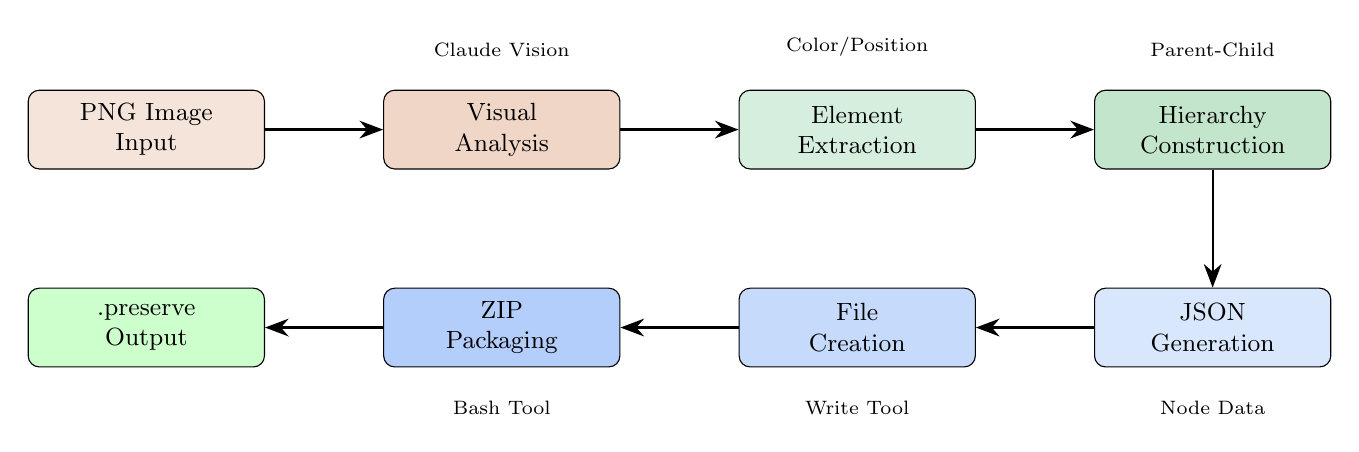
\begin{tikzpicture}[
    node distance=1.5cm,
    box/.style={rectangle, draw, rounded corners, minimum width=3cm, minimum height=1cm, align=center, font=\small},
    arrow/.style={-{Stealth[length=3mm]}, thick},
    label/.style={font=\scriptsize, align=center}
]

% Nodes
\node[box, fill=claudecolor!20] (png) {PNG Image\\Input};
\node[box, fill=claudecolor!30, right=of png] (vision) {Visual\\Analysis};
\node[box, fill=processcolor!20, right=of vision] (extract) {Element\\Extraction};
\node[box, fill=processcolor!30, right=of extract] (structure) {Hierarchy\\Construction};
\node[box, fill=filecolor!20, below=of structure] (json) {JSON\\Generation};
\node[box, fill=filecolor!30, left=of json] (files) {File\\Creation};
\node[box, fill=filecolor!40, left=of files] (zip) {ZIP\\Packaging};
\node[box, fill=green!20, left=of zip] (preserve) {.preserve\\Output};

% Arrows
\draw[arrow] (png) -- (vision);
\draw[arrow] (vision) -- (extract);
\draw[arrow] (extract) -- (structure);
\draw[arrow] (structure) -- (json);
\draw[arrow] (json) -- (files);
\draw[arrow] (files) -- (zip);
\draw[arrow] (zip) -- (preserve);

% Labels
\node[label, above=0.3cm of vision] {Claude Vision};
\node[label, above=0.3cm of extract] {Color/Position};
\node[label, above=0.3cm of structure] {Parent-Child};
\node[label, below=0.3cm of json] {Node Data};
\node[label, below=0.3cm of files] {Write Tool};
\node[label, below=0.3cm of zip] {Bash Tool};

\end{tikzpicture}
\caption{PNG to .preserve Conversion Pipeline}
\end{figure}

\subsection{Tool Calls Summary}

\begin{table}[H]
\centering
\begin{tabular}{@{}clll@{}}
\toprule
\textbf{Step} & \textbf{Tool} & \textbf{Purpose} & \textbf{Output} \\
\midrule
1 & Read (image) & Load PNG for visual analysis & Image data \\
2 & Glob/Grep & Explore .preserve format spec & Format knowledge \\
3 & Read & Study existing node types & Node structure \\
4 & Write & Create directory structure & Folders \\
5 & Write & Generate JSON files & JSON documents \\
6 & Bash (zip) & Package into archive & .preserve file \\
\bottomrule
\end{tabular}
\caption{Tool Invocations in Conversion Process}
\end{table}

% =============================================================================
\section{Stage 1: Visual Analysis}
% =============================================================================

\subsection{Tool Call: Read (Image File)}

The first step is loading the PNG image for visual analysis. Claude's multimodal capabilities allow direct interpretation of raster images.

\begin{lstlisting}[language=bash, title=Tool Invocation]
Tool: Read
Parameters: {
  "file_path": "/path/to/presets-screen.png"
}
\end{lstlisting}

\subsection{Visual Processing}

When Claude reads an image file, the following analysis occurs:

\begin{enumerate}
    \item \textbf{Global Layout Recognition}
    \begin{itemize}
        \item Device frame identification (iPhone 16 Pro: 393×852)
        \item Content area boundaries
        \item Grid/alignment detection
    \end{itemize}

    \item \textbf{Element Identification}
    \begin{itemize}
        \item Rectangular regions (frames, cards, buttons)
        \item Text elements (labels, headings, body text)
        \item Icons and decorative elements
        \item Background colors and fills
    \end{itemize}

    \item \textbf{Color Extraction}
    \begin{itemize}
        \item Dominant colors (background: \texttt{\#000000})
        \item Accent colors (green: \texttt{\#618538})
        \item Text colors (white: \texttt{\#FFFFFF}, gray: \texttt{\#8E8E93})
        \item UI element colors (cards: \texttt{\#1A1A1A})
    \end{itemize}

    \item \textbf{Spatial Relationships}
    \begin{itemize}
        \item Nesting hierarchy (which elements contain others)
        \item Relative positioning (x, y offsets from parent)
        \item Dimensions (width, height of each element)
    \end{itemize}
\end{enumerate}

\subsection{Data Extraction Example}

From visual analysis of the "Presets" screen:

\begin{lstlisting}[language=json, title=Extracted Element Data]
{
  "element": "Search Bar",
  "visual_observations": {
    "position": "top of content area, below status bar",
    "approximate_y": 59,
    "width": "full width with padding",
    "height": "approximately 36px",
    "background_color": "dark gray (#1C1C1E)",
    "corner_radius": "10px (pill shape)",
    "contains": [
      { "type": "icon", "content": "magnifying glass", "color": "#8E8E93" },
      { "type": "text", "content": "Search presets", "color": "#8E8E93" }
    ]
  }
}
\end{lstlisting}

% =============================================================================
\section{Stage 2: Format Specification Research}
% =============================================================================

\subsection{Tool Calls: Glob and Grep}

Before generating the .preserve file, the codebase is explored to understand the exact format specification.

\begin{lstlisting}[language=bash, title=Format Discovery]
# Find existing .preserve handling code
Tool: Glob
Parameters: { "pattern": "**/*preserve*" }

# Search for node type definitions
Tool: Grep
Parameters: {
  "pattern": "PreserveNode",
  "path": "src/"
}

# Find archive structure code
Tool: Grep
Parameters: {
  "pattern": "readPreserveArchive",
  "output_mode": "content"
}
\end{lstlisting}

\subsection{Tool Calls: Read (Source Files)}

Key source files are read to understand the data structures:

\begin{lstlisting}[language=bash, title=Source File Analysis]
# Node type definitions
Tool: Read
Parameters: { "file_path": "src/preserve/types.ts" }

# Archive structure
Tool: Read
Parameters: { "file_path": "src/preserve/preserve-archive.ts" }

# Node converter (preserve -> scene graph)
Tool: Read
Parameters: { "file_path": "src/preserve/node-converter.ts" }

# Factory functions (how nodes are created)
Tool: Read
Parameters: { "file_path": "src/scene/nodes/factory.ts" }
\end{lstlisting}

\subsection{Discovered Format Specification}

From the source code analysis, the .preserve format was determined:

\begin{lstlisting}[language=text, title=.preserve Archive Structure]
archive.preserve (ZIP file)
|-- mimetype                    # "application/vnd.designlibre.preserve"
|-- document.json               # Document metadata
|-- pages/
|   |-- page-{id}.json          # Page content with node tree
|-- tokens/
|   |-- colors.json             # Design tokens
|   |-- typography.json
|-- components/
|   |-- component-{id}.json     # Reusable components
|-- assets/
|   |-- manifest.json           # Asset references
|-- prototypes/
|   |-- flows.json              # Prototype interactions
|-- history/
|   |-- changelog.json          # Version history
|-- META-INF/
    |-- container.xml           # Archive metadata
\end{lstlisting}

% =============================================================================
\section{Stage 3: Hierarchy Construction}
% =============================================================================

\subsection{Parent-Child Relationship Mapping}

Based on visual analysis, a hierarchical structure is constructed:

\begin{lstlisting}[language=text, title=Node Hierarchy]
PAGE: Presets Screen
  |
  +-- FRAME: iPhone 16 Pro (393x852)
        |
        +-- FRAME: Status Bar
        |     +-- TEXT: Time
        |     +-- FRAME: Signal Icons
        |
        +-- FRAME: Content Area
              |
              +-- FRAME: Header Row
              |     +-- TEXT: "Presets"
              |     +-- FRAME: Icons Container
              |
              +-- FRAME: Search Bar
              |     +-- TEXT: "Search presets"
              |
              +-- FRAME: Tab Bar
              |     +-- FRAME: Tab (For You)
              |     +-- FRAME: Tab (Scenes)
              |     +-- FRAME: Tab (Categories)
              |
              +-- FRAME: Preset Card
              |     +-- TEXT: Title
              |     +-- FRAME: Tags Row
              |     +-- FRAME: Play Button
              |
              +-- FRAME: Bottom Navigation
                    +-- FRAME: Nav Item (Presets)
                    +-- FRAME: Nav Item (Timer)
                    +-- FRAME: Nav Item (Settings)
\end{lstlisting}

\subsection{Node ID Generation}

Each node requires a unique identifier:

\begin{lstlisting}[language=typescript, title=ID Generation Strategy]
// Pattern used for node IDs
const generateNodeId = (descriptor: string): string => {
  // Human-readable prefix + uniqueness
  return `${descriptor}-${Date.now().toString(36)}`;
};

// Examples:
// "iphone-frame"
// "content-area"
// "search-bar"
// "preset-card-1"
\end{lstlisting}

% =============================================================================
\section{Stage 4: JSON Generation}
% =============================================================================

\subsection{PreserveNode Structure}

Each visual element is converted to a PreserveNode JSON object:

\begin{lstlisting}[language=typescript, title=PreserveNode Interface]
interface PreserveNode {
  id: string;
  type: 'FRAME' | 'TEXT' | 'VECTOR' | 'GROUP' | 'IMAGE';
  name: string;

  transform: {
    x: number;      // Position relative to parent
    y: number;
    width: number;
    height: number;
    rotation: number;
  };

  appearance?: {
    fills?: PreservePaint[];
    strokes?: PreservePaint[];
    strokeWeight?: number;
    cornerRadius?: number;
    opacity?: number;
    effects?: PreserveEffect[];
  };

  // Type-specific properties
  characters?: string;        // For TEXT nodes
  textStyle?: TextStyle;      // For TEXT nodes
  clipContent?: boolean;      // For FRAME nodes

  children?: PreserveNode[];  // Nested nodes
}
\end{lstlisting}

\subsection{Paint (Fill/Stroke) Structure}

\begin{lstlisting}[language=typescript, title=PreservePaint Interface]
interface PreservePaint {
  type: 'SOLID' | 'GRADIENT_LINEAR' | 'GRADIENT_RADIAL' | 'IMAGE';
  visible: boolean;
  opacity: number;

  // For SOLID
  color?: { r: number; g: number; b: number; a: number };

  // For gradients
  gradientStops?: Array<{
    position: number;
    color: { r: number; g: number; b: number; a: number };
  }>;
}
\end{lstlisting}

\subsection{Color Conversion}

Colors observed in the PNG are converted to normalized RGBA:

\begin{lstlisting}[language=typescript, title=Color Conversion]
// Hex to normalized RGBA
function hexToRgba(hex: string): { r: number; g: number; b: number; a: number } {
  const result = /^#?([a-f\d]{2})([a-f\d]{2})([a-f\d]{2})$/i.exec(hex);
  return {
    r: parseInt(result[1], 16) / 255,  // 0-1 range
    g: parseInt(result[2], 16) / 255,
    b: parseInt(result[3], 16) / 255,
    a: 1
  };
}

// Examples:
// #000000 -> { r: 0, g: 0, b: 0, a: 1 }
// #FFFFFF -> { r: 1, g: 1, b: 1, a: 1 }
// #618538 -> { r: 0.38, g: 0.52, b: 0.22, a: 1 }
// #1C1C1E -> { r: 0.11, g: 0.11, b: 0.12, a: 1 }
\end{lstlisting}

\subsection{Example Node Generation}

\begin{lstlisting}[language=json, title=Generated Search Bar Node]
{
  "id": "search-bar",
  "type": "FRAME",
  "name": "Search Bar",
  "transform": {
    "x": 16,
    "y": 59,
    "width": 361,
    "height": 36,
    "rotation": 0
  },
  "appearance": {
    "fills": [{
      "type": "SOLID",
      "color": { "r": 0.11, "g": 0.11, "b": 0.12, "a": 1 },
      "opacity": 1,
      "visible": true
    }],
    "cornerRadius": 10,
    "opacity": 1
  },
  "clipContent": true,
  "children": [
    {
      "id": "search-placeholder",
      "type": "TEXT",
      "name": "Search Placeholder",
      "transform": {
        "x": 36,
        "y": 9,
        "width": 100,
        "height": 18,
        "rotation": 0
      },
      "characters": "Search presets",
      "textStyle": {
        "fontFamily": "SF Pro",
        "fontSize": 15,
        "fontWeight": 400,
        "fills": [{
          "type": "SOLID",
          "color": { "r": 0.56, "g": 0.56, "b": 0.58, "a": 1 }
        }]
      }
    }
  ]
}
\end{lstlisting}

% =============================================================================
\section{Stage 5: File Creation}
% =============================================================================

\subsection{Directory Structure Creation}

\begin{lstlisting}[language=bash, title=Tool Invocations for Directory Creation]
# Create base directory
Tool: Bash
Parameters: {
  "command": "mkdir -p presets-design/{pages,tokens,components,assets,prototypes,history,META-INF}"
}
\end{lstlisting}

\subsection{File Generation Sequence}

Each file is created using the Write tool:

\begin{lstlisting}[language=bash, title=File Creation Sequence]
# 1. Mimetype (must be first, uncompressed in ZIP)
Tool: Write
Parameters: {
  "file_path": "presets-design/mimetype",
  "content": "application/vnd.designlibre.preserve"
}

# 2. Document metadata
Tool: Write
Parameters: {
  "file_path": "presets-design/document.json",
  "content": "<document JSON>"
}

# 3. Page content (main design)
Tool: Write
Parameters: {
  "file_path": "presets-design/pages/page-presets-main.json",
  "content": "<page JSON with all nodes>"
}

# 4. Design tokens
Tool: Write
Parameters: {
  "file_path": "presets-design/tokens/colors.json",
  "content": "<color tokens JSON>"
}

# 5. Additional metadata files
Tool: Write
Parameters: {
  "file_path": "presets-design/META-INF/container.xml",
  "content": "<container XML>"
}

# ... repeat for all required files
\end{lstlisting}

\subsection{Document.json Structure}

\begin{lstlisting}[language=json, title=document.json Content]
{
  "$schema": "https://designlibre.app/schemas/preserve/1.0/document.json",
  "id": "doc-presets-screen",
  "name": "Presets Screen Design",
  "version": "1.0.0",
  "created": "2026-01-03T12:00:00.000Z",
  "modified": "2026-01-03T12:00:00.000Z",
  "generator": "Claude AI",
  "generatorVersion": "1.0",
  "pages": [
    {
      "id": "page-presets-main",
      "name": "Presets Screen",
      "path": "pages/page-presets-main.json"
    }
  ],
  "settings": {
    "gridSize": 8,
    "snapToGrid": true,
    "showRulers": true
  }
}
\end{lstlisting}

% =============================================================================
\section{Stage 6: Archive Packaging}
% =============================================================================

\subsection{ZIP Creation}

The final step packages all files into a ZIP archive:

\begin{lstlisting}[language=bash, title=ZIP Packaging Command]
Tool: Bash
Parameters: {
  "command": "cd presets-design && zip -r ../presets-screen.preserve mimetype document.json pages/ tokens/ components/ assets/ prototypes/ history/ META-INF/"
}
\end{lstlisting}

\subsection{ZIP Structure Requirements}

\begin{enumerate}
    \item \textbf{Mimetype First}: The \texttt{mimetype} file must be the first entry in the ZIP archive (uncompressed) for proper MIME type detection
    \item \textbf{No Compression for Mimetype}: Use \texttt{-0} flag for mimetype if needed
    \item \textbf{Relative Paths}: All paths inside the ZIP are relative to the archive root
\end{enumerate}

\begin{lstlisting}[language=bash, title=Proper ZIP Creation (with mimetype first)]
# Create ZIP with mimetype first (uncompressed)
cd presets-design
zip -0 ../presets-screen.preserve mimetype
zip -r ../presets-screen.preserve . -x mimetype
\end{lstlisting}

% =============================================================================
\section{Complete Tool Call Sequence}
% =============================================================================

\subsection{Chronological Tool Invocations}

\begin{table}[H]
\centering
\small
\begin{tabular}{@{}clp{6cm}@{}}
\toprule
\textbf{\#} & \textbf{Tool} & \textbf{Purpose} \\
\midrule
1 & Read & Load PNG image for visual analysis \\
2 & Glob & Find .preserve-related source files \\
3 & Grep & Search for PreserveNode type definitions \\
4 & Read & Study preserve-archive.ts structure \\
5 & Read & Study node-converter.ts for data mapping \\
6 & Read & Study factory.ts for node creation \\
7 & Read & Study types.ts for interfaces \\
8 & Bash & Create directory structure \\
9 & Write & Create mimetype file \\
10 & Write & Create document.json \\
11 & Write & Create pages/page-presets-main.json \\
12 & Write & Create tokens/colors.json \\
13 & Write & Create tokens/typography.json \\
14 & Write & Create components/index.json \\
15 & Write & Create assets/manifest.json \\
16 & Write & Create prototypes/flows.json \\
17 & Write & Create history/changelog.json \\
18 & Write & Create META-INF/container.xml \\
19 & Bash & Package into ZIP archive \\
\bottomrule
\end{tabular}
\caption{Complete Tool Call Sequence}
\end{table}

% =============================================================================
\section{Data Flow Diagram}
% =============================================================================

\begin{figure}[H]
\centering
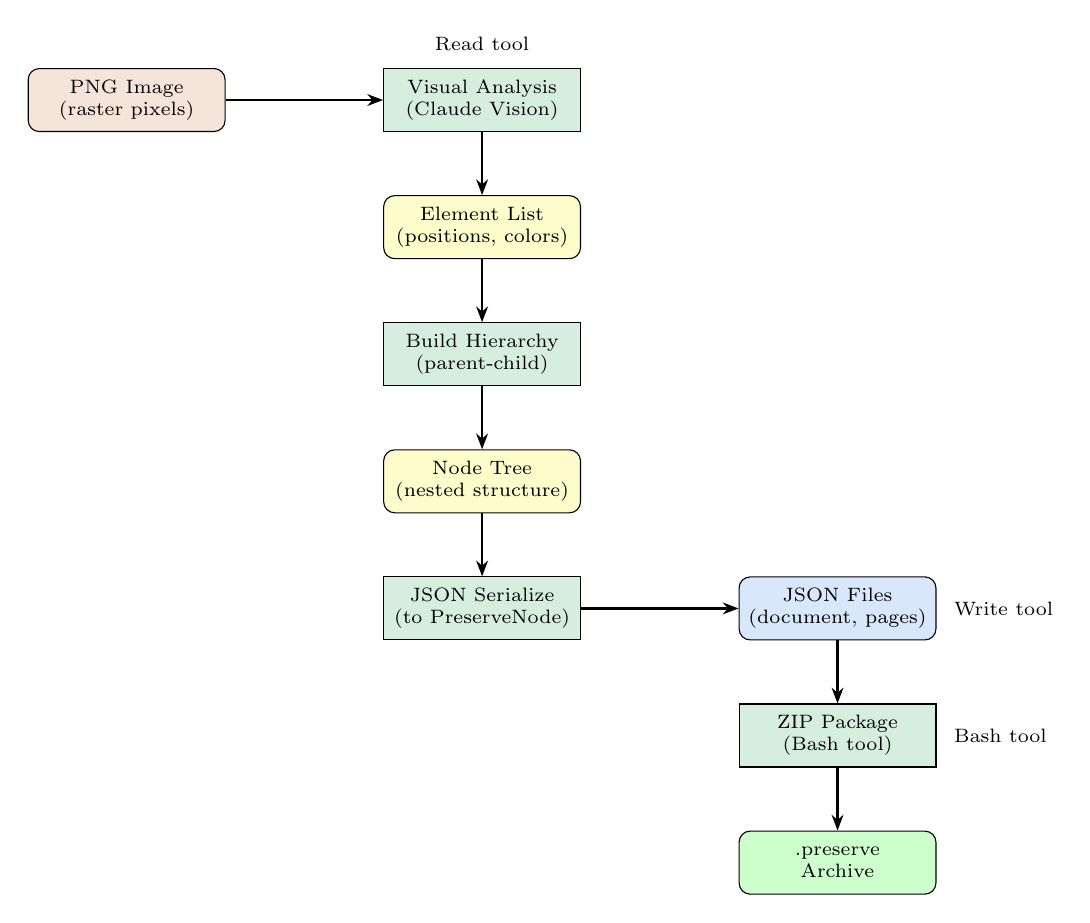
\begin{tikzpicture}[
    node distance=0.8cm,
    data/.style={rectangle, draw, rounded corners, minimum width=2.5cm, minimum height=0.8cm, align=center, font=\scriptsize},
    process/.style={rectangle, draw, fill=processcolor!20, minimum width=2.5cm, minimum height=0.8cm, align=center, font=\scriptsize},
    arrow/.style={-{Stealth[length=2mm]}, thick}
]

% Left column - Input
\node[data, fill=claudecolor!20] (png) {PNG Image\\(raster pixels)};

% Processing column
\node[process, right=2cm of png] (analyze) {Visual Analysis\\(Claude Vision)};
\node[data, fill=yellow!20, below=of analyze] (elements) {Element List\\(positions, colors)};
\node[process, below=of elements] (hierarchy) {Build Hierarchy\\(parent-child)};
\node[data, fill=yellow!20, below=of hierarchy] (tree) {Node Tree\\(nested structure)};
\node[process, below=of tree] (serialize) {JSON Serialize\\(to PreserveNode)};

% Right column - Output
\node[data, fill=filecolor!20, right=2cm of serialize] (json) {JSON Files\\(document, pages)};
\node[process, below=of json] (package) {ZIP Package\\(Bash tool)};
\node[data, fill=green!20, below=of package] (preserve) {.preserve\\Archive};

% Arrows
\draw[arrow] (png) -- (analyze);
\draw[arrow] (analyze) -- (elements);
\draw[arrow] (elements) -- (hierarchy);
\draw[arrow] (hierarchy) -- (tree);
\draw[arrow] (tree) -- (serialize);
\draw[arrow] (serialize) -- (json);
\draw[arrow] (json) -- (package);
\draw[arrow] (package) -- (preserve);

% Labels
\node[font=\scriptsize, above=0.1cm of analyze] {Read tool};
\node[font=\scriptsize, right=0.1cm of json] {Write tool};
\node[font=\scriptsize, right=0.1cm of package] {Bash tool};

\end{tikzpicture}
\caption{Data Flow Through Conversion Pipeline}
\end{figure}

% =============================================================================
\section{Limitations and Considerations}
% =============================================================================

\subsection{Manual Analysis Limitations}

\begin{enumerate}
    \item \textbf{Approximate Measurements}: Positions and dimensions are estimated from visual inspection, not pixel-perfect
    \item \textbf{Font Detection}: Font families are inferred (e.g., "SF Pro" for iOS) rather than extracted
    \item \textbf{Color Sampling}: Colors are approximated from visual observation
    \item \textbf{No OCR}: Text content is read visually, not through OCR
    \item \textbf{Complex Shapes}: Intricate vector paths cannot be perfectly recreated
\end{enumerate}

\subsection{Format Fidelity}

\begin{table}[H]
\centering
\begin{tabular}{@{}lcc@{}}
\toprule
\textbf{Property} & \textbf{Accuracy} & \textbf{Method} \\
\midrule
Position (x, y) & $\pm$5px & Visual estimation \\
Dimensions & $\pm$5px & Visual estimation \\
Colors (solid) & High & Color picker approximation \\
Corner radius & Medium & Visual estimation \\
Font size & $\pm$2px & Visual estimation \\
Text content & High & Manual transcription \\
Hierarchy & High & Logical grouping \\
\bottomrule
\end{tabular}
\caption{Property Extraction Accuracy}
\end{table}

\subsection{Potential Improvements}

For automated PNG import, the following enhancements could be implemented:

\begin{enumerate}
    \item \textbf{Computer Vision}: Use edge detection and segmentation for precise boundaries
    \item \textbf{OCR Integration}: Extract text content programmatically
    \item \textbf{Color Extraction}: Sample exact pixel colors from the image
    \item \textbf{AI Segmentation}: Use Claude Vision API with structured output for element detection
    \item \textbf{Template Matching}: Recognize common UI patterns (buttons, inputs, cards)
\end{enumerate}

% =============================================================================
\section{Conclusion}
% =============================================================================

The PNG to .preserve conversion process involves six distinct stages:

\begin{enumerate}
    \item \textbf{Visual Analysis}: Claude's multimodal capabilities interpret the raster image
    \item \textbf{Format Research}: Source code exploration reveals the .preserve specification
    \item \textbf{Hierarchy Construction}: Visual elements are organized into a parent-child tree
    \item \textbf{JSON Generation}: Each element becomes a PreserveNode with transform and appearance
    \item \textbf{File Creation}: JSON documents are written to the required directory structure
    \item \textbf{Archive Packaging}: Files are compressed into a ZIP with .preserve extension
\end{enumerate}

The toolchain leverages Claude's ability to:
\begin{itemize}
    \item Read and interpret image files visually
    \item Search and understand source code for format specifications
    \item Generate structured JSON data from visual observations
    \item Execute file system operations through tool calls
\end{itemize}

This process transforms an opaque raster image into an editable, hierarchical design document that can be opened and modified in DesignLibre.

\end{document}
